\documentclass[11pt]{article}
\usepackage[margin=1in]{geometry}
\usepackage{amsmath,amssymb,amsthm}
\usepackage{graphicx}
\graphicspath{{../figures/}}
\usepackage{xcolor}
\usepackage{booktabs}
\usepackage[numbers,sort&compress]{natbib}
\usepackage{xurl}
\usepackage[colorlinks=true,linkcolor=blue!50!black,citecolor=blue!50!black,urlcolor=blue!50!black]{hyperref}

\theoremstyle{remark}
\newtheorem{remark}{Remark}

\newcommand{\dd}{\mathrm{d}}
\newcommand{\eps}{\varepsilon}

\title{The instability of ghost-scalar wormholes\\at large dimension}
\author{Nathan Moinvaziri\thanks{\href{mailto:nathan@nathanm.com}{nathan@nathanm.com}}\\[2pt]
\normalsize\textit{Independent researcher}}
\date{October 2026}

\begin{document}
\maketitle

\begin{abstract}
The static, massless, reflection-symmetric wormhole supported by a ghost scalar field (the Ellis--Bronnikov
wormhole) has exactly one unstable radial mode, and in $D$ spacetime dimensions its growth rate $W$ has been computed
numerically. We derive its large-$D$ expansion by matched asymptotic expansions:
\[
W^2a^2 = 2(D-3) - 4\ln 2 + \frac{\pi^2/3+4\ln^2 2}{D-3} + O(D^{-2}),
\]
with $a$ the throat radius. The first two terms are obtained in closed form. The third is a matching integral evaluated
to ten digits and identified by an integer-relation search. The master equation is written in the gauge in which the
scalar is unperturbed; two independent integrations of it reproduce the published eigenvalues to nine or more
significant figures and confirm the expansion up to $D=1000$, with a remainder of order $D^{-2}$. At large $D$ the throat moves
rigidly while the mode lives in the nearly flat region outside it, with the profile
$\delta r\propto (r/a)\,e^{1-r^2/a^2}$. Because the wormhole is the critical solution of the threshold between collapse
to a black hole and inflationary expansion, $1/W$ is also the slope of the logarithmic lifetime law there. Published
evolutions in four, five and six dimensions are consistent with it.
\end{abstract}

\tableofcontents

\section{Introduction}

A traversable wormhole needs matter that violates the null energy condition at its throat~\cite{MT1988}. The
simplest example is the wormhole of Ellis and Bronnikov~\cite{Ellis1973,Bronnikov1973}, held open by a massless scalar
field with the wrong sign of kinetic energy (a ghost). It is unstable. González, Guzmán and Sarbach proved that its
spherically symmetric perturbations have exactly one exponentially growing mode~\cite{GGS2009a}, and evolutions show
that, perturbed, the throat either collapses to a black hole or expands into an inflating region~\cite{SH2002,GGS2009b}.
Torii and Shinkai found the same single unstable mode in every dimension they computed, $D=4$--$11$, $20$, $50$ and
$100$, and noted that the instability becomes faster as $D$ grows~\cite{TS2013}.

How fast? A fit to their largest-$D$ values gives roughly $W^2a^2\approx2D-8.6$, but no formula has been given. The question is
natural for the large-$D$ expansion of general relativity~\cite{EST2013}, in which the gravitational field of a compact
object is confined to a thin layer near its horizon. Here the layer is the region near the throat where the geometry
differs from flat space, of width $a/D$.

This paper derives the large-$D$ expansion of $W$ and the shape of the unstable mode. Section~\ref{sec:setup} writes
the perturbation problem as a single master equation. Section~\ref{sec:numerics} solves it numerically and compares with
Ref.~\cite{TS2013}. Section~\ref{sec:largeD} carries out the matched expansion, and Sec.~\ref{sec:mode} describes the
mode. Section~\ref{sec:threshold} turns the growth rate into a prediction for the lifetime of near-threshold
evolutions and compares it with published runs.

\section{The wormhole and its radial perturbations}\label{sec:setup}

In $D=n+2$ dimensions, with $G_{ab}=\kappa T_{ab}$ and a ghost scalar,
$T_{ab}=-\left(\partial_a\phi\,\partial_b\phi-\tfrac12 g_{ab}(\partial\phi)^2\right)$, the static, massless,
reflection-symmetric wormhole is ultrastatic~\cite{TS2013}:
\begin{equation}
\dd s^2=-\dd t^2+\dd l^2+r(l)^2\,\dd\Omega_n^2,\qquad r'^2=1-\left(\frac{a}{r}\right)^{2(n-1)},\qquad
\kappa\phi'^2=\frac{n(n-1)\,a^{2(n-1)}}{r^{2n}},\label{eq:bg}
\end{equation}
with $l\in\mathbb R$, the throat $r=a$ at $l=0$, and primes denoting $\dd/\dd l$. Since $g_{tt}=-1$, $t$ is proper time
everywhere.

For spherically symmetric perturbations we write
\begin{equation}
\dd s^2=-e^{2\nu}\dd t^2+e^{2\lambda}\dd l^2+(r+\delta r)^2\dd\Omega_n^2,\qquad
(\nu,\lambda,\delta r)=(N,\Lambda,Y)(l)\,e^{Wt},
\end{equation}
in the gauge $\delta\phi=0$, which is available everywhere because $\phi'$ never vanishes. Linearizing the Einstein
equations, written for the warped product of the $(t,l)$ plane with the $n$-sphere, and the scalar equation gives:
\begin{itemize}
\item from the $tl$ equation, $\Lambda=Y'/r'$;
\item from the scalar equation, $N=\Lambda-nY/r$, after a reparametrization of $t$ removes an
  integration function of $t$;
\item from the angular equation, the master equation
\begin{equation}
Y''-\left(\frac{2r''}{r'}+\frac{n\,r'}{r}\right)Y'+\left(\frac{n\,r'^2}{r^2}+\frac{r''}{r}\right)Y=W^2Y.\label{eq:master}
\end{equation}
\end{itemize}
With these, the $tt$ and $ll$ equations hold identically. The throat is a regular singular point of
Eq.~\eqref{eq:master} with exponents $0$ and $3$; the mode that moves the throat is the even one, normalized by
$Y(0)=1$, and a growing mode ($W>0$) must decay as $l\to\pm\infty$.

Since $\dd/\dd l=r'\,\dd/\dd r$, the metric perturbation $\Lambda=Y'/r'$ is simply $\dd Y/\dd r$. On either side of the
throat, with $F(r)=r'^2=1-(a/r)^{2(n-1)}$, Eq.~\eqref{eq:master} becomes the first-order system
\begin{equation}
\frac{\dd Y}{\dd r}=\Lambda,\qquad
F\,r\,\frac{\dd\Lambda}{\dd r}=W^2rY+\Lambda\left(\frac{rF_r}{2}+nF\right)-\frac{nFY}{r}-\frac{F_rY}{2},\label{eq:system}
\end{equation}
regular-singular at $r=a$, where $F=0$. The even mode is the solution analytic in $r-a$. Where $F=1$ to exponential
accuracy, Eq.~\eqref{eq:system} reduces to $Y''-(n/r)Y'+(n/r^2)Y=W^2Y$, whose decaying solution is
\begin{equation}
Y_{\rm far}=r^{(n+1)/2}\,K_{(n-1)/2}(Wr).\label{eq:far}
\end{equation}

\section{The numerical spectrum}\label{sec:numerics}

We solved the eigenvalue problem in two ways. The first integrates Eq.~\eqref{eq:master} in $l$ from a series start
at the throat and shoots on the decay at large $l$. It is accurate to about $10^{-3}$ for $D\le10$, but its start near
the throat loses accuracy at large $D$, where the near-throat layer is thin. The second integrates
Eq.~\eqref{eq:system} in $r$ from a Frobenius series at $r=a$ to $r_m=a\,e^{X/s}$, $s=2(D-3)$, where $F=1-e^{-X}$, and
matches $\Lambda/Y$ there to the logarithmic derivative of Eq.~\eqref{eq:far}. Changing $X$ from 40 to 50, the
starting point and the tolerances moves $W^2a^2$ by $4\times10^{-10}$ at $D=20$ and $1.5\times10^{-6}$ at $D=1000$.

Both find exactly one growing mode. The second reproduces Torii and Shinkai's values~\cite{TS2013}, obtained with a
different, gauge-invariant master variable, to nine or more significant figures (Table~\ref{tab:W}).

\begin{table}[t]
\centering
\caption{$W^2a^2$ for the growing mode. For $D\le11$ the values are Torii and Shinkai's~\cite{TS2013}; for $D\ge20$
they are from the $r$-integration of Sec.~\ref{sec:numerics}, with Ref.~\cite{TS2013} in parentheses where available.
The last columns compare with the three-term expansion~\eqref{eq:result}.}
\label{tab:W}
\begin{tabular}{rlrr}
\toprule
$D$ & $W^2a^2$ & relative difference from \eqref{eq:result} & (difference)$\times s^2$ \\
\midrule
4 & 1.39705243 & $2.2$ & $-12$ \\
5 & 2.98495893 & $0.28$ & $-14$ \\
6 & 4.68662054 & $5.9\times10^{-2}$ & $-10$ \\
7 & 6.46258414 & $1.05\times10^{-2}$ & $-4.3$ \\
8 & 8.28975936 & $2.4\times10^{-3}$ & $2.0$ \\
10 & 12.04426501 & $6.0\times10^{-3}$ & $14$ \\
20 & 31.5751101276 (31.5751101285) & $1.3\times10^{-3}$ & $48$ \\
50 & 91.3457759034 (91.3457759137) & $8.2\times10^{-5}$ & $66$ \\
100 & 191.2830176842 (191.2830177297) & $9.8\times10^{-6}$ & $71$ \\
200 & 391.2543342170 & $1.2\times10^{-6}$ & $72.6$ \\
500 & 991.2379714266 & $7.5\times10^{-8}$ & $73.0$ \\
1000 & 1991.2326553188 & $8.4\times10^{-9}$ & $66\pm6$ \\
\bottomrule
\end{tabular}
\end{table}

\section{The large-\texorpdfstring{$D$}{D} expansion}\label{sec:largeD}

Set $a=1$, $s=2(D-3)$, $\eps=1/s$, and write $W^2=s+\Omega$ with $\Omega=\Omega_0+\eps\,\Omega_1+\dots$. Near the throat
we use $R=r^s$, so that $F=1-1/R$ and $r=e^{\eps\ln R}$. Equation~\eqref{eq:system} becomes, exactly,
\begin{equation}
Y_R=\eps\,\frac{\Lambda r}{R},\qquad
(R-1)\Lambda_R=(1+\eps\Omega)\,rY+\frac{\Lambda}{2R}+\left(\tfrac12+\eps\right)\frac{\Lambda(R-1)}{R}
-\left(\tfrac12+\eps\right)\frac{Y(R-1)}{Rr}-\frac{Y}{2rR}.\label{eq:near}
\end{equation}
Expanding $Y=\sum\eps^kY_k$ and $\Lambda=\sum\eps^k\Lambda_k$ gives at each order
\begin{equation}
(R-1)\Lambda_k'-\tfrac12\Lambda_k=h_k(R),\label{eq:order}
\end{equation}
where $h_k$ depends on lower orders. The solution analytic at the throat is
\begin{equation}
\Lambda_k=-2h_k(1)+(R-1)^{1/2}\int_1^R\frac{h_k(R')-h_k(1)}{(R'-1)^{3/2}}\,\dd R'.\label{eq:sol}
\end{equation}
At large $R$ it contains $G_kR^{1/2}$, with
\begin{equation}
G_k=\int_1^\infty\frac{h_k(R)-h_k(1)}{(R-1)^{3/2}}\,\dd R.
\end{equation}
But $R^{1/2}=r^{D-3}$ is the far zone's growing solution, the one that Eq.~\eqref{eq:far} excludes. A growing mode
therefore requires $G_k=0$ at every order, and this fixes $\Omega$.

\paragraph{Orders 0 and 1.} At order 0, $h_0=Y_0/2$ and $Y_0$ is constant; we normalize $Y_0=1$, so $\Lambda_0=-1$. At
order 1,
\begin{equation}
h_1=\Omega_0+\ln R-\frac{2(R-1)}{R},\qquad \Lambda_1=-2\Omega_0-2\ln R,\qquad Y_1=-\ln R.
\end{equation}
Here $G_1=0$ identically, because $\int_1^\infty\ln R\,(R-1)^{-3/2}\dd R=2\pi=\int_1^\infty2(R-1)^{-1/2}R^{-1}\dd R$.

\paragraph{Order 2.} Then $Y_2=-2\Omega_0\ln R-\tfrac32\ln^2R$ and
\begin{equation}
h_2=\Omega_1-\frac{2\Omega_0(R-1)}{R}-\Omega_0\ln R-2\ln^2R,\qquad G_2=-4\pi\Omega_0-2J,
\end{equation}
with, substituting $R=1+u^2$ and integrating by parts once,
\begin{equation}
J=\int_1^\infty\frac{\ln^2R}{(R-1)^{3/2}}\,\dd R=8\int_0^\infty\frac{\ln(1+u^2)}{1+u^2}\,\dd u=8\pi\ln2 .
\end{equation}
So $G_2=0$ gives
\begin{equation}
\Omega_0=-4\ln2.
\end{equation}
Consistently, the solution~\eqref{eq:sol} at this order is
\begin{equation}
\Lambda_2=-2\Omega_1+2\Omega_0\ln R+4\ln^2R-8\Omega_0\,u\arctan u-16\,u\,K(u),
\end{equation}
with $u=\sqrt{R-1}$ and $K(u)=\int_0^u\ln(1+t^2)\,(1+t^2)^{-1}\,\dd t$,
and its $R^{1/2}$ term, $-(4\pi\Omega_0+16\pi\ln2)\,u$, vanishes for the same $\Omega_0$.

\paragraph{Order 3.} $Y_3$, $h_3$ and $G_3$ follow in the same way. $\Omega_1$ enters $h_3$ only through
$-\Omega_1[\ln R+2(R-1)/R]$, so $G_3=G_3|_{\Omega_1=0}-4\pi\Omega_1$. We evaluated $G_3$ on a grid in $v=\sqrt{\ln R}$,
in which every integrand is smooth, with cumulative Simpson integration on three grids. The two finer grids agree to
$10^{-9}$ and give
\begin{equation}
\Omega_1=10.4233603788 .
\end{equation}
An integer-relation search (PSLQ~\cite{PSLQ1999}) over $\{\Omega_1,\pi^2,\ln^22,\ln2,1\}$ at tolerance $10^{-9}$ returns
$3\Omega_1-2\pi^2-24\ln^22=0$, that is $\Omega_1=2\pi^2/3+8\ln^22=10.42336037874$, which differs from the computed value
by $6\times10^{-11}$. We regard this closed form as an identification, not a derivation.

\paragraph{Result.} With $s=2(D-3)$,
\begin{equation}
\boxed{\;W^2a^2=2(D-3)-4\ln2+\frac{\pi^2/3+4\ln^22}{D-3}+O(D^{-2}).\;}\label{eq:result}
\end{equation}
Table~\ref{tab:W} and Fig.~\ref{fig:main}(a) compare it with the numerical eigenvalues. The difference times $s^2$
settles near $73$ at $D=200$--$500$, as an $O(D^{-2})$ remainder should; at $D=1000$ it is $66\pm6$, within that
value's numerical uncertainty. The three terms are within $1.1\%$ of the exact value at $D=7$--$11$ and at every larger $D$
computed, and within $10^{-5}$ (relative) at $D=100$. At $D=4$ they are not useful.

\paragraph{Matching.} The far solution~\eqref{eq:far}, expanded in the overlap $1\ll R\ll e^s$, has logarithmic derivative
$\Lambda/Y=-1-\eps(2\Omega_0+3\ln R)+O(\eps^2)$, and so does the near-zone solution. The matching at this order holds for
any $\Omega$; the condition on $\Omega$ comes only from the absence of the growing term.

\begin{figure}[t]
\centering
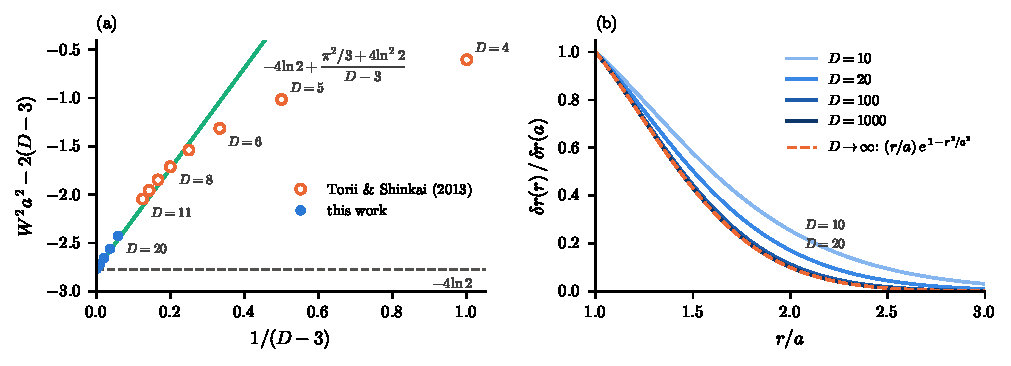
\includegraphics[width=\textwidth]{fig6_wormhole_largeD.pdf}
\caption{(a) $W^2a^2-2(D-3)$ against $1/(D-3)$: Torii and Shinkai's eigenvalues~\cite{TS2013} for $D=4$--$11$ (open
circles) and this work's for $D=20$--$2000$ (filled), with the two-term (dashed) and three-term (solid) large-$D$
results~\eqref{eq:result}. (b) The profile $\delta r(r)/\delta r(a)$ of the growing mode for $D=10$, $20$, $100$ and
$1000$, and its large-$D$ limit $(r/a)\,e^{1-r^2/a^2}$ (dashed).}
\label{fig:main}
\end{figure}

\section{The shape of the mode}\label{sec:mode}

The expansion also says where the instability lives. In the layer near the throat, of width $a/(D-3)$ in $r$, the
perturbation is constant to leading order, $Y=Y_0$: the throat moves as a whole, and $\Lambda/Y=\delta r'/\delta r=-1/a$
at the outer edge of the layer. Outside, the geometry is flat up to terms of order $(a/r)^{2(D-3)}$, and the mode is the
decaying solution~\eqref{eq:far}. For $x=Wr$ of order $\nu^{1/2}$, $\nu=(D-3)/2$, the Bessel function behaves as
$K_\nu(x)\propto x^{-\nu}e^{-x^2/4\nu}\left[1+O(\nu^{-1})\right]$, so to leading order
\begin{equation}
\frac{\delta r(r)}{\delta r(a)}=\frac{r}{a}\,e^{1-r^2/a^2},
\end{equation}
which has slope $-1/a$ at $r=a$, as the near zone requires. Figure~\ref{fig:main}(b) shows the numerical profiles
approaching this limit.

So at large $D$ the instability is a mode of nearly flat space outside a rigidly moving throat, which acts as a boundary
with the fixed condition $\delta r'/\delta r=-1/a$. It extends over a radius of order $a$, not over the thin layer of
width $a/D$ in which the wormhole's geometry is concentrated.

\section{Consequence for the collapse--expansion threshold}\label{sec:threshold}

Shinkai and Hayward evolved the four-dimensional wormhole with Gaussian pulses of either sign of energy and found a
sharp boundary between collapse to a black hole and inflationary expansion, which they called ``a new kind of critical
behaviour reminiscent of that found by Choptuik''~\cite{SH2002}. Near it the final black-hole mass tends to a finite
value and the time before the outcome grows logarithmically. Both are the signatures of type I critical
phenomena~\cite{GMG2007}, whose critical solution is static with exactly one unstable mode. The ghost wormhole is such a
solution~\cite{GGS2009a,TS2013}. The time spent near it is then
\begin{equation}
T\simeq\frac{1}{W}\ln\frac{1}{|p-p_*|}+\text{const},\label{eq:lifetime}
\end{equation}
with $p$ the family parameter and $p_*$ its threshold value; $W$ is the growth rate in proper time at the throat.

Refs.~\cite{SH2002,ST2017} use the null coordinate $x^-=(t-r_*)/\sqrt2$, in which a proper-time interval at fixed
position is $\Delta x^-=\Delta t/\sqrt2$. Their threshold is at zero injected energy, and $\Delta E$ is proportional to
the distance from it: linear in the amplitude of a ghost pulse, and quadratic in that of a normal pulse, which perturbs
the metric only at second order. The predicted slope of
the horizon's formation coordinate $x^-_H$ against $\ln(1/\Delta E)$ is therefore $1/(\sqrt2\,W)$. Table~\ref{tab:life}
compares it with the published runs.

\begin{table}[t]
\centering
\caption{Slope of $x^-_H/a$ against $\ln(1/\Delta E)$ near the threshold. Predicted: $1/(\sqrt2\,Wa)$ from
Table~\ref{tab:W}. Measured: Shinkai and Hayward's fitted exponent~\cite{SH2002}, and two-run slopes from the
$\alpha_{\rm GB}=0$ rows of Shinkai and Torii's Table~I~\cite{ST2017}, with uncertainties from the rounding of that
table.}
\label{tab:life}
\begin{tabular}{rlllll}
\toprule
$D$ & $1/(Wa)$ & predicted & measured & source & runs \\
\midrule
4 & 0.846 & 0.598 & 0.60 (ghost), 0.61 (normal) & \cite{SH2002} & fit \\
4 & & & $0.71\pm0.14$ & \cite{ST2017} & $\Delta E/a=0.03$, $0.10$ \\
5 & 0.579 & 0.409 & $0.43\pm0.02$ & \cite{ST2017} & $\Delta E/a=0.15$, $0.61$ \\
6 & 0.462 & 0.327 & $0.335\pm0.011$ & \cite{ST2017} & $\Delta E/a=0.38$, $1.50$ \\
\bottomrule
\end{tabular}
\end{table}

The agreement in $D=4$ is with Shinkai and Hayward's fit over two decades of $\Delta E$; the comparison with the
linear growth rate does not appear in Refs.~\cite{SH2002,GGS2009a}. The higher-dimensional runs of Ref.~\cite{ST2017} were not designed to measure the lifetime
law, and two runs at moderate amplitude give only a rough slope, but in $D=5$ and $6$ they agree with the prediction
within their uncertainties. A bisection to the threshold in $D=5$ and $6$, with the lifetime fitted against
$\ln|p-p_*|$, would test Eq.~\eqref{eq:lifetime} properly. At large $D$ the prediction is
$T\simeq a\ln(1/|p-p_*|)/\sqrt{2(D-3)}$.

\section{Discussion}\label{sec:discussion}

Equation~\eqref{eq:result} answers how the ghost wormhole's instability depends on dimension: its rate grows as
$\sqrt{2(D-3)}/a$, with corrections $-4\ln2$ and $(\pi^2/3+4\ln^22)/(D-3)$ to $W^2a^2$. The leading behaviour has a
simple reading. Outside a thin layer the wormhole is flat space, and the mode is the lowest one of flat space with the
throat as a boundary. The constant $-4\ln2$ comes from the layer itself, through the single integral $J$.

The analysis covers radial perturbations of the massless, reflection-symmetric member of the static family only. The
asymmetric members (different asymptotic masses on the two sides) also have a single unstable mode~\cite{GGS2009a},
and the same near-zone/far-zone construction should apply to them. Charged wormholes, wormholes supported by a ghost
with a potential, and non-spherical perturbations are not considered.

We have not found an analytic expression for this growth rate, or a large-$D$ analysis of these wormholes, in the
literature we searched: Refs.~\cite{TS2013,ST2017,GGS2009a,GGS2009b,SH2002}, the recent evolution of
Ref.~\cite{XCY2025}, and searches for large-$D$ treatments of wormhole stability. This is not an exhaustive survey.

\section{How the results were obtained}\label{sec:method}

The author set the question and scope and reviewed each stage; Anthropic's Claude, run as an agent with a Python
environment, did the literature reading, derivations, code and drafting. No claim rests on the assistant's word alone:
\begin{itemize}
\item \emph{Master equation.} The reduction of the linearized Einstein--scalar equations to Eq.~\eqref{eq:master} and
the identities for the remaining components were checked symbolically (SymPy), with a control in which a wrong
coefficient leaves nonzero residuals.
\item \emph{Spectrum.} Two independent integrations, compared with the published table of Ref.~\cite{TS2013}, which
uses a different master variable.
\item \emph{Expansion.} Each closed form at orders 1 and 2 was checked by quadrature; $\Omega_1$ was computed on three
grids and identified by PSLQ, and the expansion was compared with the numerical eigenvalues up to $D=1000$.
\item \emph{Numbers.} Every number in the tables and text is recomputed by one script from the data files, with
checks that fail if a stated agreement does not hold.
\end{itemize}
These checks are internal; the work has not yet been reviewed by specialists.

\paragraph{Reproducibility.} The derivation and integration scripts, the data behind the figure and the number checks
are in \texttt{notes/wormhole\_largeD/} of the accompanying repository, \url{https://github.com/nmoinvaz/negative-mass},
and the figure is made by \texttt{paper/figures/make\_figures.py}.

\paragraph{Acknowledgments.} The author thanks Anthropic's Claude, which carried out the analysis, computations and
drafting described in Sec.~\ref{sec:method} under the author's direction.

\begin{thebibliography}{99}

\bibitem{MT1988} M. S. Morris and K. S. Thorne, ``Wormholes in spacetime and their use for interstellar travel: a tool
for teaching general relativity,'' Am. J. Phys. \textbf{56}, 395 (1988), doi:10.1119/1.15620.
\bibitem{Ellis1973} H. G. Ellis, ``Ether flow through a drainhole: a particle model in general relativity,'' J. Math.
Phys. \textbf{14}, 104 (1973), doi:10.1063/1.1666161.
\bibitem{Bronnikov1973} K. A. Bronnikov, ``Scalar-tensor theory and scalar charge,'' Acta Phys. Pol. B \textbf{4}, 251
(1973).
\bibitem{GGS2009a} J. A. González, F. S. Guzmán and O. Sarbach, ``Instability of wormholes supported by a ghost scalar
field. I. Linear stability analysis,'' Class. Quantum Grav. \textbf{26}, 015010 (2009), arXiv:0806.0608.
\bibitem{SH2002} H. Shinkai and S. A. Hayward, ``Fate of the first traversible wormhole: black-hole collapse or
inflationary expansion,'' Phys. Rev. D \textbf{66}, 044005 (2002), arXiv:gr-qc/0205041.
\bibitem{GGS2009b} J. A. González, F. S. Guzmán and O. Sarbach, ``Instability of wormholes supported by a ghost scalar
field. II. Nonlinear evolution,'' Class. Quantum Grav. \textbf{26}, 015011 (2009), arXiv:0806.1370.
\bibitem{TS2013} T. Torii and H. Shinkai, ``Wormholes in higher dimensional space-time: exact solutions and their
linear stability analysis,'' Phys. Rev. D \textbf{88}, 064027 (2013), arXiv:1309.2058.
\bibitem{EST2013} R. Emparan, R. Suzuki and K. Tanabe, ``The large $D$ limit of general relativity,'' JHEP
\textbf{06}, 009 (2013), arXiv:1302.6382.
\bibitem{PSLQ1999} H. R. P. Ferguson, D. H. Bailey and S. Arno, ``Analysis of PSLQ, an integer relation finding
algorithm,'' Math. Comp. \textbf{68}, 351 (1999).
\bibitem{GMG2007} C. Gundlach and J. M. Martín-García, ``Critical phenomena in gravitational collapse,'' Living Rev.
Relativ. \textbf{10}, 5 (2007), arXiv:0711.4620.
\bibitem{ST2017} H. Shinkai and T. Torii, ``Nonlinear dynamics in the Einstein--Gauss--Bonnet gravity,'' Phys. Rev. D
\textbf{96}, 044009 (2017), arXiv:1706.02070.
\bibitem{XCY2025} A. Xu, X. Y. Chew and D. Yeom, ``Dynamics of Bronnikov--Ellis wormhole with double-null simulation,''
JCAP \textbf{08} (2025) 012, arXiv:2503.07610.

\end{thebibliography}

\end{document}
